\documentclass[11pt]{beamer}
\usetheme{Goettingen}
\usepackage[utf8]{inputenc}
\usepackage[english]{babel}
\usefonttheme{professionalfonts}
\usepackage{amsmath}
\usepackage{amsfonts}
\usepackage{amssymb}
\usepackage{graphicx}
\usepackage{array}
\newcolumntype{P}[1]{>{\centering\arraybackslash}p{#1}}

\newenvironment{tightcenter}{%
  \setlength\topsep{0pt}
  \setlength\parskip{0pt}
  \begin{center}
}{%
  \end{center}
}

\author[P.Herruzo]{Pedro Herruzo}
\title[Master thesis]{\textbf{Grad-CAM}:\\
\textbf{Visual Explanations from Deep Networks via Gradient-based Localization } \\
Ramprasaath R. Selvaraju, Michael Cogswell, Abhishek Das, Ramakrishna Vedantam, Devi Parikh, Dhruv Batra}
%\setbeamercovered{transparent} 
%\setbeamertemplate{navigation symbols}{} 
%\logo{} 
%\institute{} 
%\date{} 
%subject{Recommenders} 
\setbeamerfont{page number in head/foot}{size=\medium}
\setbeamertemplate{footline}[frame number]
\begin{document}

\begin{frame}
\titlepage
\end{frame}

\begin{frame}
\tableofcontents
\end{frame}

\section{Introduction}
\begin{frame}{Introduction (I)}

Nowadays deeper means better:

\begin{figure}
    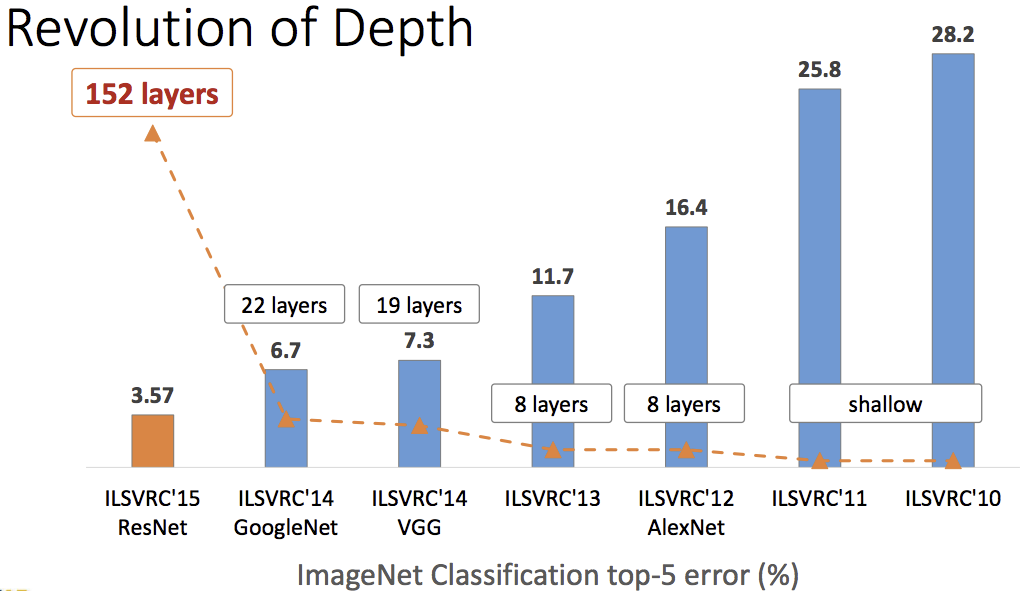
\includegraphics[width=1.05\textwidth]{deep_revolution.png}
\end{figure}

\end{frame}

\begin{frame}{Introduction (II)}

By using deep models, we \textbf{sacrifice interpretable modules} for uninterpretable ones that achieve \textbf{greater performance} through greater abstraction (more layers) and tighter integration (end-to-end training).

\begin{figure}
    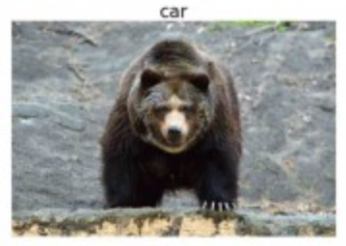
\includegraphics[width=.5\textwidth]{car.png}
\end{figure}

When models fail, they fail spectacularly disgracefully, without warning or explanation, leaving a user staring at an incoherent output, wondering why.

\end{frame}

\begin{frame}{Introduction (III)}
Interpretability Matters:

\begin{itemize}
\item[•] When AI is \textbf{significantly weaker than humans} and not yet reliably 'deployable' (e.g., visual question answering), the goal of transparency and explanations is to\textbf{ identify the failure modes}, thereby helping researchers focus their efforts on the most fruitful research directions.
\item[•] When AI is \textbf{on par with humans} and reliably 'deployable' (e.g., image classification), the goal is to \textbf{establish appropriate trust and confidence in users}.
\item[•] When AI is \textbf{significantly stronger than humans} (e.g., chess or Go), the goal of explanations is in \textbf{machine teaching} (i.e., a machine teaching a human about how to make better decisions).
\end{itemize}
\end{frame}

\begin{frame}{Introduction (IV)}
What do we want?
\begin{figure}
    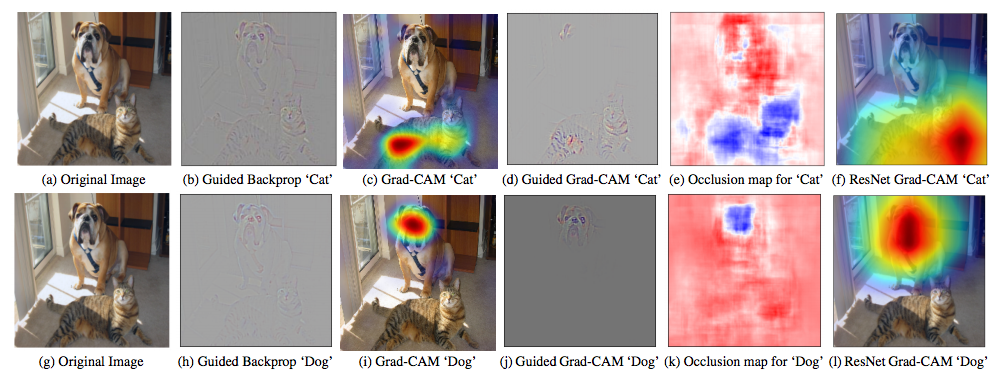
\includegraphics[width=1.05\textwidth]{first.png}
\end{figure}
\end{frame}

\section{Related work}


\frame{\tableofcontents[currentsection]}

%%%%%%%%%%%%%%%%%%%%%%%%%% New related work
\subsection{2010: Freeze weights and learn the input}
\begin{frame}{}
%%%%%%%%%%%%%%%%%%%%%%%%%% tile and authors
\begin{tightcenter}
\textbf{Understanding Representations Learned in Deep Architectures}
\\
Dumitru Erhan, Aaron Courville, and Yoshua Bengio
\end{tightcenter}
$\newline$
They propose two methods: First, Sampling from top to down using that layers $j -1$ and $j$ form an RBM from which they can sample using block Gibbs sampling. Second, their new idea: maximizing the activation of a unit as an optimization problem fixing the parameters after training the network and learning the input image:
\begin{figure}
    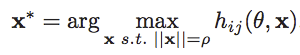
\includegraphics[width=.50\textwidth]{1_max1.png}
\end{figure}

Beyond that, they also explore the invariance manifolds for each of the hidden units w.r.t the target class:
\begin{figure}
    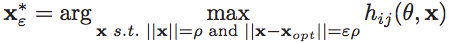
\includegraphics[width=.70\textwidth]{1_max2.png}
\end{figure}
\end{frame}

\begin{frame}{2010: Freeze weights and learn the input (II)}
\begin{figure}
    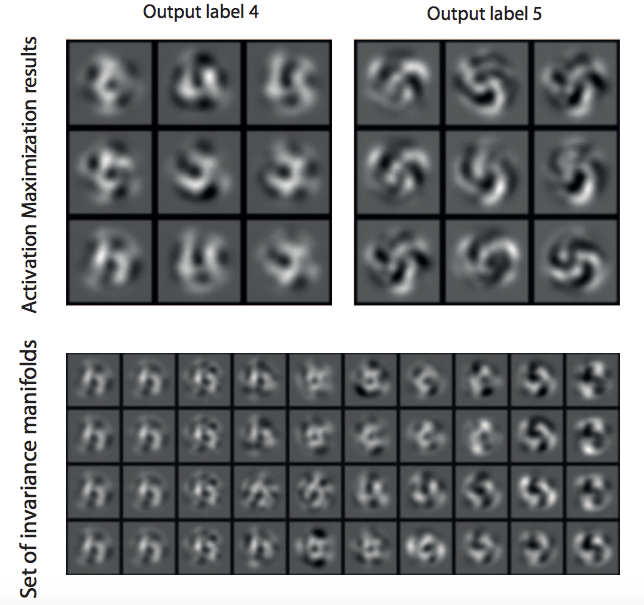
\includegraphics[width=.80\textwidth]{1_results.png}
\end{figure}
\end{frame}


%%%%%%%%%%%%%%%%%%%%%%%%%% New related work
\subsection{2013: Deconvolutions and patch occlusions}
\begin{frame}{}
%%%%%%%%%%%%%%%%%%%%%%%%%% tile and authors
\begin{tightcenter}
\textbf{Visualizing and Understanding Convolutional Networks}
\\
Matthew D. Zeiler, Rob Fergus
\end{tightcenter}
$\newline$
They propose two methods: First, Up sampling top-down and computing the transpose of a convolution (deconvolution):
\begin{figure}
    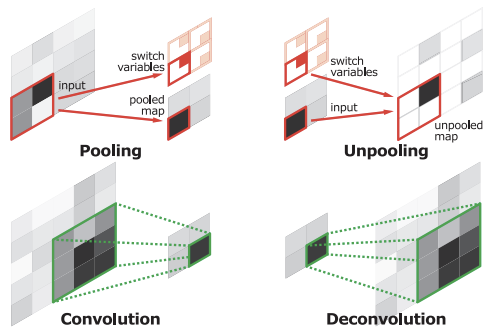
\includegraphics[width=.80\textwidth]{2_1_deconvolution.png}
\end{figure}
\end{frame}

\begin{frame}{2013: Deconvolutions and patch occlusions (II)}

Second, they perturb inputs by occluding patches and classifying the occluded image, typically resulting in lower classification scores for relevant objects when those objects are occluded:
\begin{figure}
    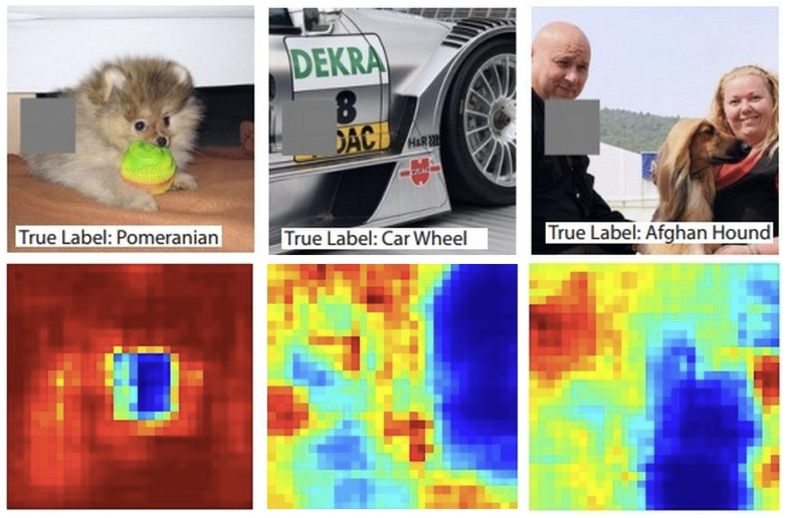
\includegraphics[width=.80\textwidth]{2_1_patches.png}
\end{figure}
\end{frame}


%%%%%%%%%%%%%%%%%%%%%%%%%% New related work - 3
\subsection{2014: Class saliency map using backprop}
\begin{frame}{}
%%%%%%%%%%%%%%%%%%%%%%%%%% tile and authors
\begin{tightcenter}
\textbf{Deep Inside Convolutional Networks: Visualising Image Classification Models and Saliency Maps}
\\
Karen Simonyan, Andrea Vedaldi,  Andrew Zisserman
\end{tightcenter}
$\newline$
They propose three methods: First, they establish connection between the gradient-based ConvNet visualisation methods and deconvolutional networks. In short, they differ just in how backpropagate the non-liniarities (i.e., ReLu).

$\newline$
Second, they generate an image by maximizing the activation of a unit in the last layer of a CNN very similarly to Bengio in 2010. More formally, let $S_c(I)$ be the score of the class $c$, computed by the classification layer of the ConvNet for an image $I$. We would like to find an $L_2$-regularised image, such that the score $S_c$ is high:
\begin{figure}
    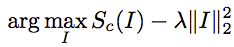
\includegraphics[width=.40\textwidth]{3_2014.png}
\end{figure}
\end{frame}

\begin{frame}{2014: Class saliency map using backprop (II)}
Creating this results:
\begin{figure}
    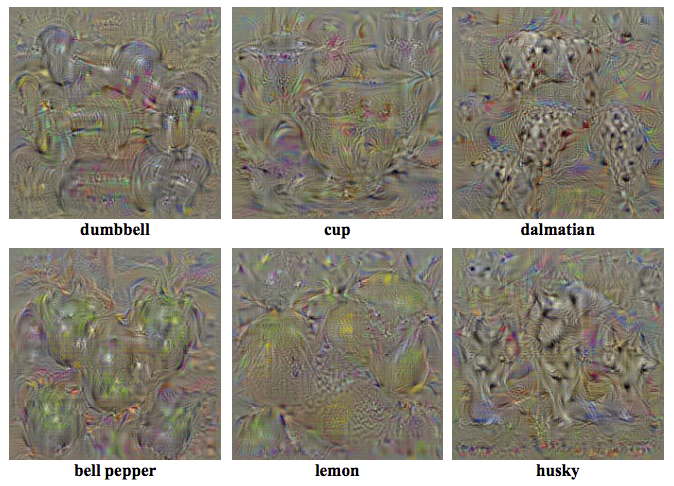
\includegraphics[width=.90\textwidth]{3_1_max_results.png}
\end{figure}
\end{frame}

\begin{frame}{2014: Class saliency map using backprop (III)}
Third, they presented a new method based on backpropagate the importance of each pixel from a target class.  Consider the linear score model for the class c
\begin{figure}
    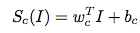
\includegraphics[width=.280\textwidth]{3_2.png}
\end{figure}
Here is easy to see that the magnitude of elements of $w$ defines the importance of the corresponding pixels of $I$ for the class $c$. In a CNN we can we approximate $S_c(I)$ with a linear function in the neighbourhood of $I_0$ by computing the first-order Taylor expansion:
\begin{figure}
    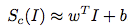
\includegraphics[width=.25\textwidth]{3_3.png}
\end{figure}
Where here the weights are just computed with backprop:
\begin{figure}
    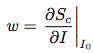
\includegraphics[width=.18\textwidth]{3_4.png}
\end{figure}
\end{frame}

\begin{frame}{2014: Class saliency map using backprop (IV)}
Creating this results:
\begin{figure}
    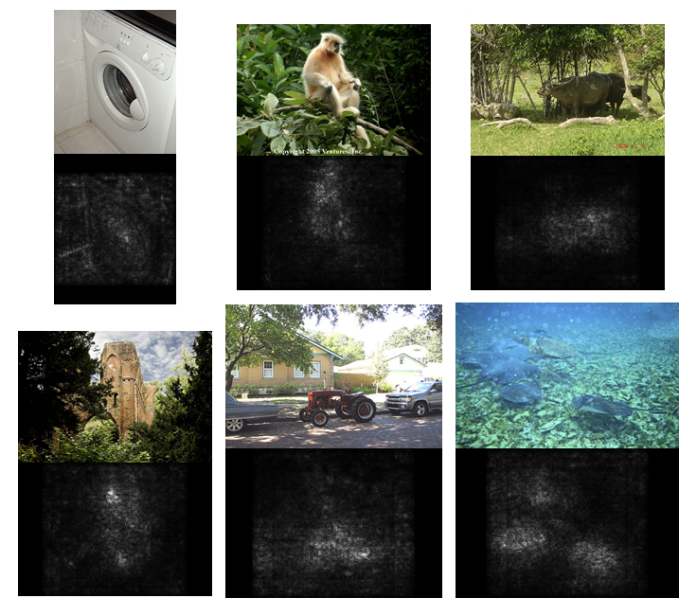
\includegraphics[width=.80\textwidth]{3_5.png}
\end{figure}
\end{frame}


%%%%%%%%%%%%%%%%%%%%%%%%%% New related work - 4
\subsection{2015: Guided backpropagation}
\begin{frame}{}
%%%%%%%%%%%%%%%%%%%%%%%%%% tile and authors
\begin{tightcenter}
\textbf{Guided backpropagation}
\\
Jost Tobias Springenberg, Alexey Dosovitskiy, Thomas Brox, Martin Riedmiller
\end{tightcenter}
$\newline$
They propose two methods: A new architecture that consists solely of convolutional layers. Second, they  add an additional guidance signal from the higher layers to usual backprop:
\begin{figure}
    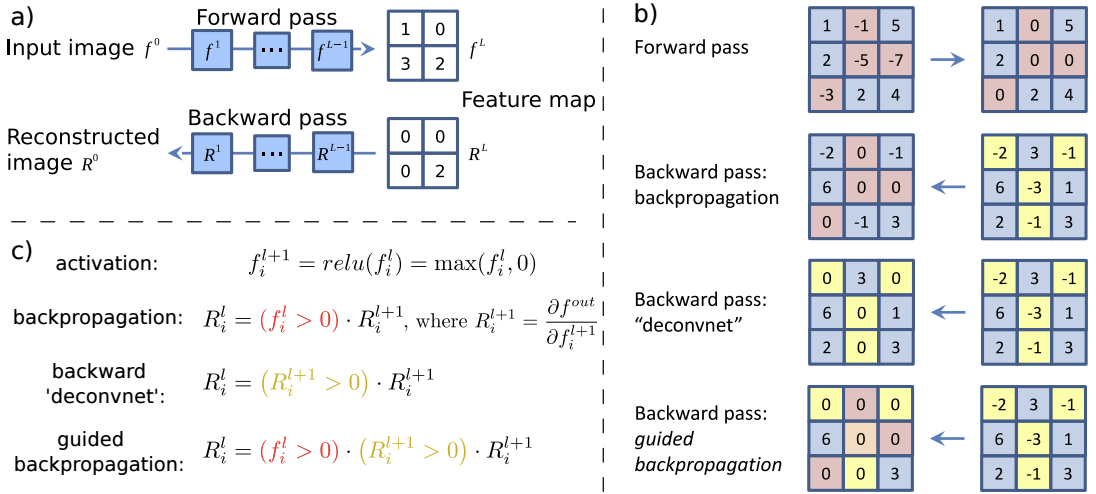
\includegraphics[width=1.\textwidth]{4_guided_backprop.png}
\end{figure}
\end{frame}

\begin{frame}{2015: Guided backpropagation (II)}

Creating this results:
\begin{figure}
    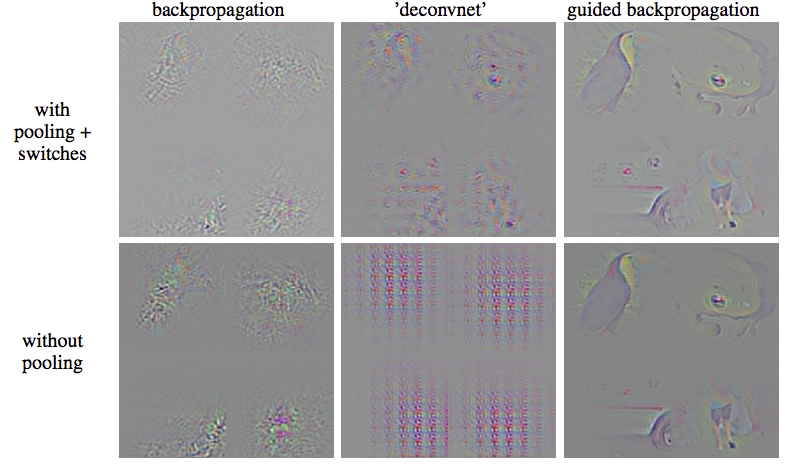
\includegraphics[width=1.\textwidth]{4_1_guided_backprop.png}
\end{figure}
\end{frame}


%%%%%%%%%%%%%%%%%%%%%%%%%% New related work - 5
\subsection{2016: Backprop to intermediate layers}
\begin{frame}{}
%%%%%%%%%%%%%%%%%%%%%%%%%% tile and authors
\begin{tightcenter}
\textbf{DISTINCT CLASS SALIENCY MAPS FOR MULTIPLE OBJECT IMAGES}
\\
Wataru Shimoda, Keiji Yanai
\end{tightcenter}
$\newline$
They propose three methods: Using CNN derivatives with respect to feature maps of the intermediate convolutional layers with up-sampling, instead of an input image as it is done by Simonyan:
\begin{figure}
    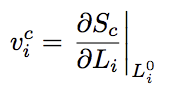
\includegraphics[width=.2\textwidth]{5_5_distincs_saliency_maps.png}
\end{figure}

Second, aggregating multiple-scale class saliency maps to compensate lower resolution of the feature maps.
\end{frame}

\begin{frame}{2016: Backprop to intermediate layers (II)}

Creating this results:
\begin{figure}
    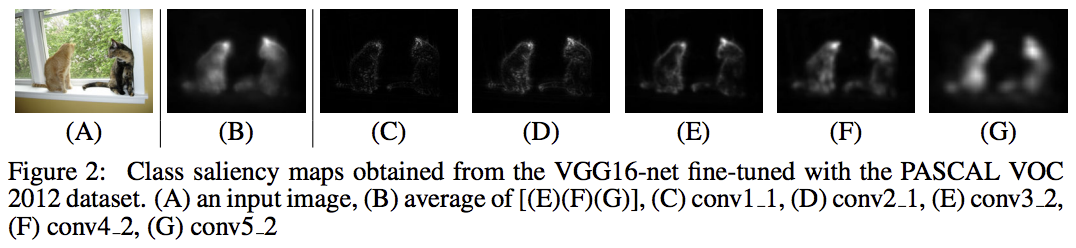
\includegraphics[width=1.05\textwidth]{5_1.png}
\end{figure}

Third, subtracting saliency maps of the other classes from saliency maps of the target class to differentiate target objects from other objects:
\begin{figure}
    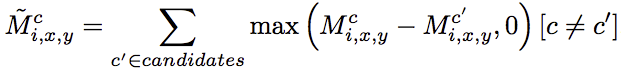
\includegraphics[width=.8\textwidth]{5_2.png}
\end{figure}
\end{frame}

\begin{frame}{2016: Backprop to intermediate layers (III)}

Creating this results:
\begin{figure}
    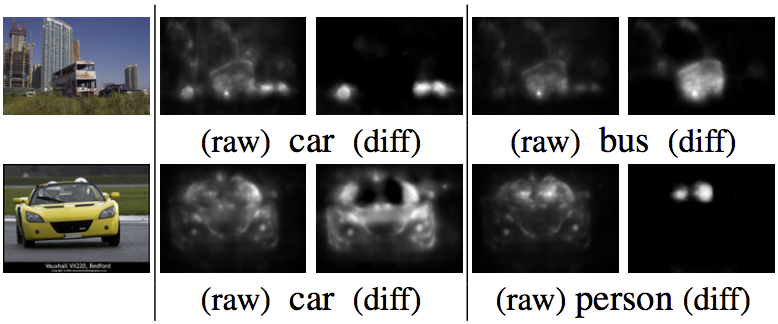
\includegraphics[width=.9\textwidth]{5_3.png}
\end{figure}

\begin{figure}
    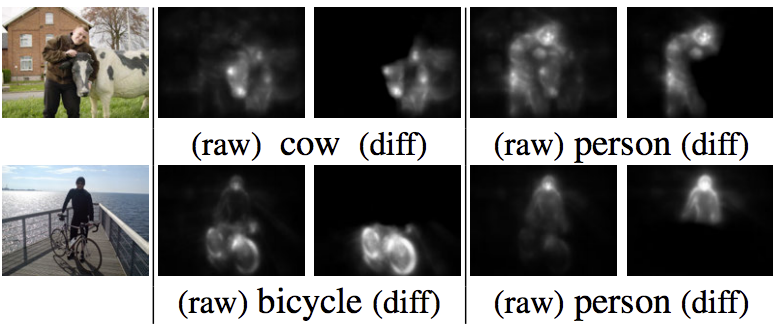
\includegraphics[width=.9\textwidth]{5_4.png}
\end{figure}
\end{frame}

%%%%%%%%%%%%%%%%%%%%%%%%%% New related work - 6
\subsection{2016: CAM from GAP}
\begin{frame}{}
%%%%%%%%%%%%%%%%%%%%%%%%%% tile and authors
\begin{tightcenter}
\textbf{DISTINCT CLASS SALIENCY MAPS FOR MULTIPLE OBJECT IMAGES}
\\
Bolei Zhou, Aditya Khosla, Agata Lapedriza, Aude Oliva, Antonio Torralba
\end{tightcenter}
$\newline$
They revisit the global average pooling layer proposed in "Network In Network" (2014), and shed light on how it explicitly enables the CNNs to have remarkable localization ability despite being trained on imagelevel labels:
\begin{figure}
    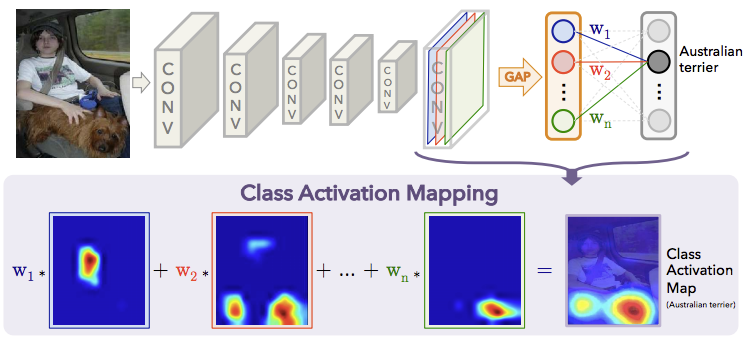
\includegraphics[width=.95\textwidth]{6_cam.png}
\end{figure}
\end{frame}


%%%%%%%%%%%%%%%%%%%%%%%%%% METHODOLOGY
\section{Methodology}

\frame{\tableofcontents[currentsection]}

\begin{frame}{Methodology (I)}
The way I see it, this method is a mix of CAM (from Agata), and backpropagate from a target class $y^c$ to the last (and hence, more abstract) convolutional layer (from Simonyan).

$\newline$
First, they compute the importance of a kernel $k$ in the last convolutional layer from the target class $y^c$ to the activation produced by this kernel $A^k$:
\begin{figure}
    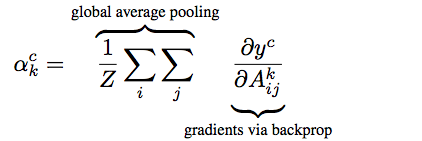
\includegraphics[width=.5\textwidth]{g1.png}
\end{figure}

Second, they use the weighted kernels activation, only the positive part, which indeed is the one that could increase the score of $y^c$:
\end{frame}


\begin{frame}{Methodology (II)}
\begin{figure}
    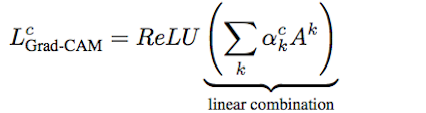
\includegraphics[width=.5\textwidth]{g2.png}
\end{figure}
After that, we just need to up-sampling to the image size. 

$\newline$
The authors show that these technique is indeed a generalization of CAM. However, with grad-CAM $y^c$ can be any differentiable activation including words from a caption or the answer to a question. Also, grad-CAM can be combined with guided-backprop in order to get high-definition discriminative visual explanations.
\end{frame}

\begin{frame}{Methodology (III)}
Grad-CAM as discriminative and guided-backprop as high-definition for any kind of problem:
\begin{figure}
    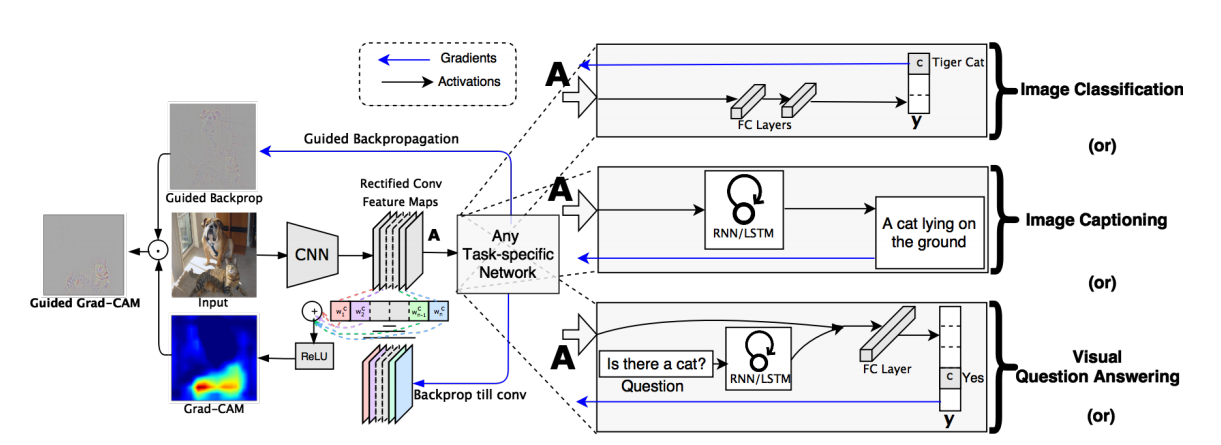
\includegraphics[width=1.05\textwidth]{g3.png}
\end{figure}
\end{frame}



%%%%%%%%%%%%%%%%%%%%%%%%%% RESULTS
\section{Results}

\frame{\tableofcontents[currentsection]}

\subsection{Localization}
\begin{frame}{Evaluating Localization and classification}
Evaluation of the localization capability
of Grad-CAM in the context of image classification over the ImageNet localization challenge which requires to provide bounding boxes in addition to classification labels:

\begin{figure}
    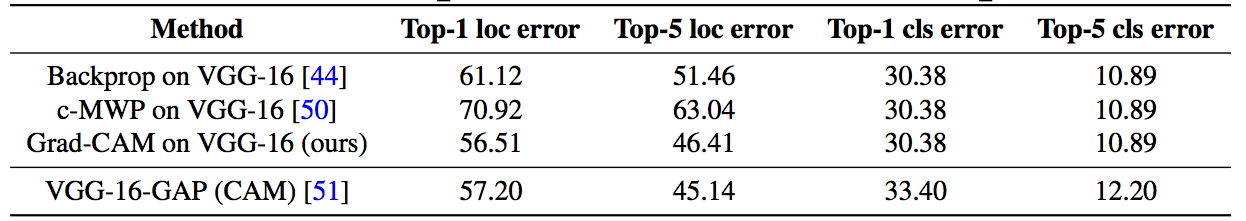
\includegraphics[width=1.\textwidth]{g4.png}
\end{figure}
\end{frame}

\subsection{Class discrimination and trustful}
\begin{frame}{Evaluating class discrimination and trustful}
In which of the following models will you trust more?

\begin{figure}
    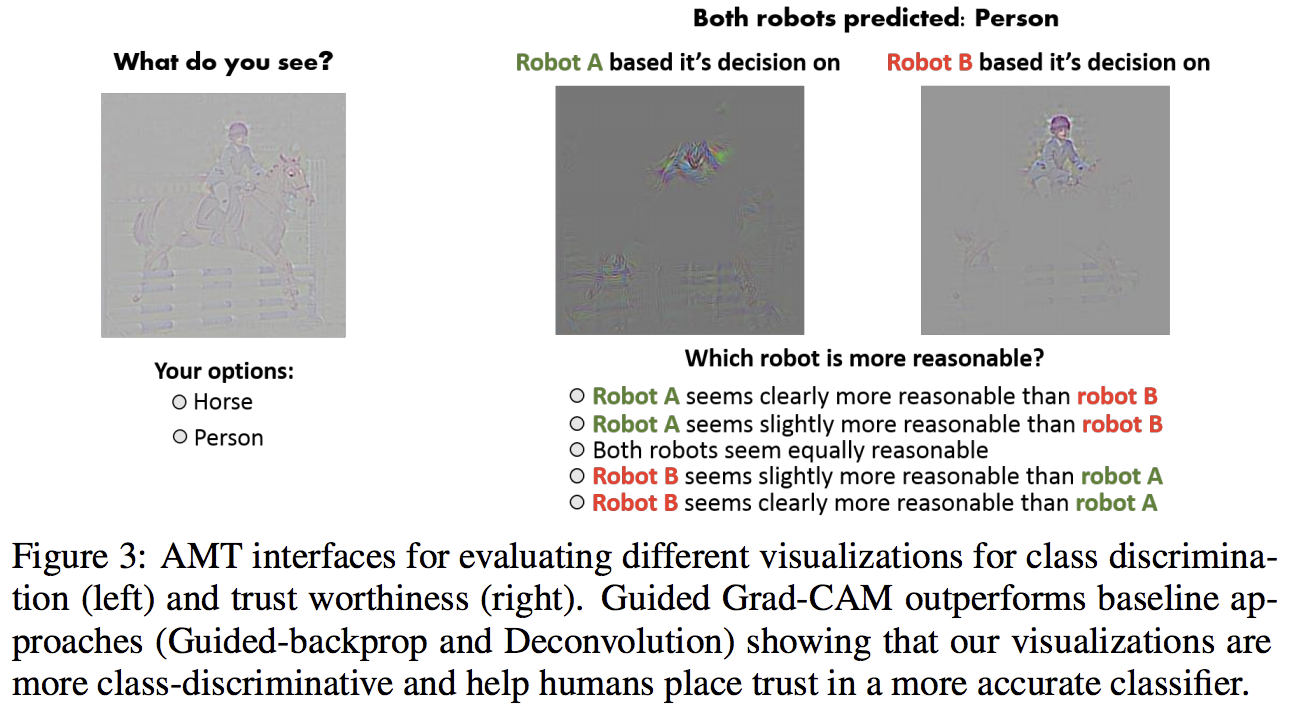
\includegraphics[width=1.05\textwidth]{g5.png}
\end{figure}
\end{frame}


\subsection{Bias in dataset}
\begin{frame}{Discovering bias in dataset}
They finetune an ImageNet trained VGG-16 model for the task of classifying “doctor” vs. “nurse” which did not generalize as well (82\%). Grad-CAM visualizations of the model predictions revealed that the model had learned to look at the person’s face/hairstyle to distinguish nurses from doctors, thus learning a gender stereotype. Indeed, in the training dataset 78\% of images for doctors were men, and 93\% images for nurses were women. Grad-CAM discovered it:

\begin{figure}
    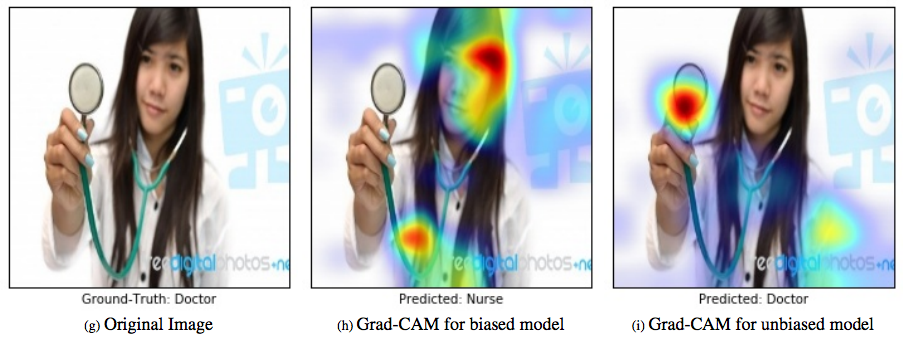
\includegraphics[width=1.\textwidth]{g6.png}
\end{figure}
\end{frame}

\subsection{Counterfactual Explanations}
\begin{frame}{Counterfactual Explanations}
Which are the regions that would make the network change
its decision more?
\begin{figure}
    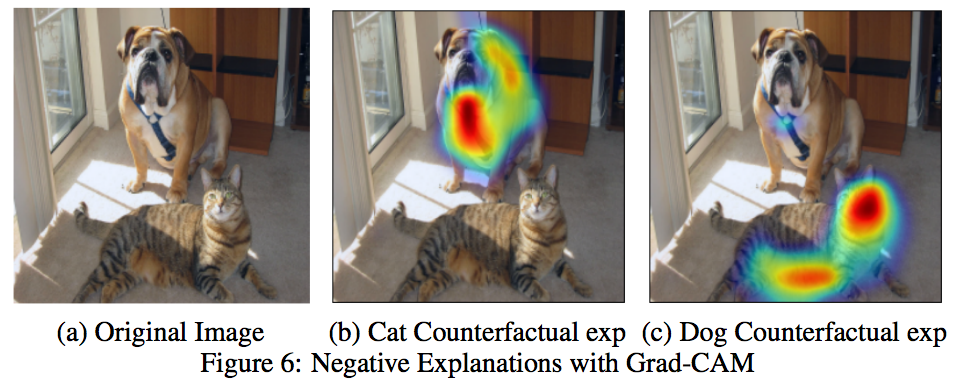
\includegraphics[width=1.05\textwidth]{g7.png}
\end{figure}
Gradient negations finds locations that drops the score:
\begin{figure}
    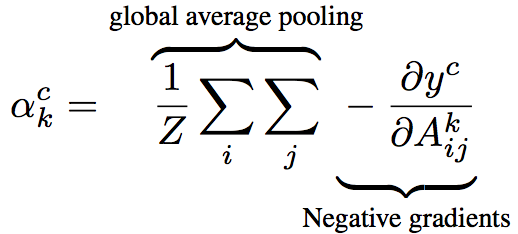
\includegraphics[width=.35\textwidth]{g8.png}
\end{figure}
\end{frame}

\subsection{Image captioning}
\begin{frame}{Image captioning}
\begin{figure}
    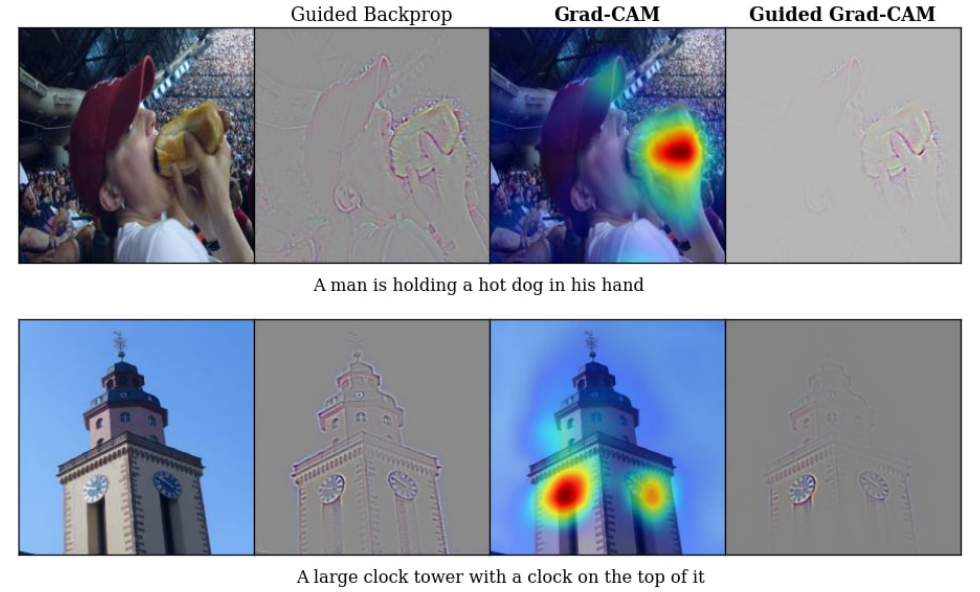
\includegraphics[width=1.05\textwidth]{g9.png}
\end{figure}
\end{frame}

\subsection{Visual QA}
\begin{frame}{Visual Question Answering}
\begin{figure}
    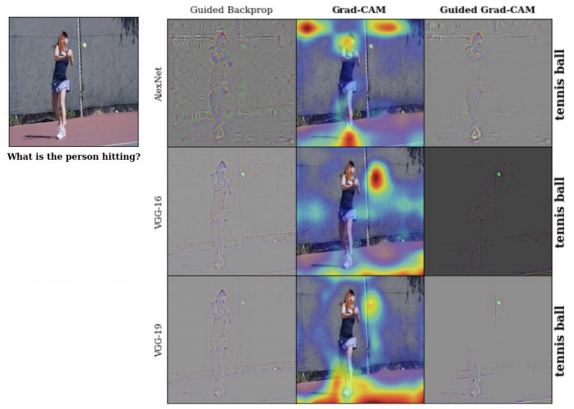
\includegraphics[width=1.05\textwidth]{g10.png}
\end{figure}
\end{frame}

%%%%%%%%%%%%%%%%%%%%%%%%%% pro/cons and future
\section{Pros/cons \& Future Work}

\frame{\tableofcontents[currentsection]}

\begin{frame}{Pros/cons \& Future Work}

Pros: It is a very general model which uses almost everything I mentioned today and applies to almost all kind of problems. It is easy to use, cheap, and transparent.

$\newline$
Cons: To really understand this method there are a bunch of previous method that you should master before.

$\newline$
Future work: Following the lines of the papers shown today, I will try to improve the current grad-CAM adding:
\begin{itemize}
\item Aggregating Grad-CAM visualizations over different layers, not just relying in the last one.
\item Subtracting Grad-CAM of the other classes from Grad-CAM of the target class to differentiate target objects from other objects.
\end{itemize}
\end{frame}

\section{}
\begin{frame}{}
\begin{figure}
    
\includegraphics[width=.8\textwidth]{last.png}
\end{figure}
\end{frame}



\end{document}